\documentclass[conference]{IEEEtran}
\IEEEoverridecommandlockouts
% The preceding line is only needed to identify funding in the first footnote. If that is unneeded, please comment it out.
\usepackage{cite}
\usepackage{amsmath,amssymb,amsfonts}
\usepackage{algorithmic}
\usepackage{graphicx}
\usepackage{textcomp}
\usepackage{xcolor}
\def\BibTeX{{\rm B\kern-.05em{\sc i\kern-.025em b}\kern-.08em
    T\kern-.1667em\lower.7ex\hbox{E}\kern-.125emX}}

\ifCLASSINFOpdf
\else
    \usepackage[dvips]{graphicx}
\fi
\usepackage{url}
\usepackage{listings}
% \usepackage[margin=1in]{geometry}
\usepackage{amsmath,amsthm,amssymb}
\usepackage{amsmath,amsthm,amssymb}
\usepackage[spanish]{babel} %Castellanización
\usepackage[T1]{fontenc} %escribe lo del teclado
\usepackage[utf8]{inputenc} %Reconoce algunos símbolos
\usepackage{lmodern} %optimiza algunas fuentes
\usepackage{blkarray}
\graphicspath{ {images/} }
\usepackage{hyperref} % Uso de links

\newcommand{\N}{\mathbb{N}}
\newcommand{\Z}{\mathbb{Z}}
\usepackage{float}
\newenvironment{theorem}[2][Theorem]{\begin{trivlist}
\item[\hskip \labelsep {\bfseries #1}\hskip \labelsep {\bfseries #2.}]}{\end{trivlist}}
\newenvironment{lemma}[2][Lemma]{\begin{trivlist}
\item[\hskip \labelsep {\bfseries #1}\hskip \labelsep {\bfseries #2.}]}{\end{trivlist}}
\newenvironment{exercise}[2][Exercise]{\begin{trivlist}
\item[\hskip \labelsep {\bfseries #1}\hskip \labelsep {\bfseries #2.}]}{\end{trivlist}}
\newenvironment{problem}[2][Problem]{\begin{trivlist}
\item[\hskip \labelsep {\bfseries #1}\hskip \labelsep {\bfseries #2.}]}{\end{trivlist}}
\newenvironment{question}[2][Question]{\begin{trivlist}
\item[\hskip \labelsep {\bfseries #1}\hskip \labelsep {\bfseries #2.}]}{\end{trivlist}}
\newenvironment{corollary}[2][Corollary]{\begin{trivlist}
\item[\hskip \labelsep {\bfseries #1}\hskip \labelsep {\bfseries #2.}]}{\end{trivlist}}
\newcommand*{\defeq}{\stackrel{\text{def}}{=}}
\newenvironment{solution}{\begin{proof}[Solution]}{\end{proof}}
\hyphenation{op-tical net-works semi-conduc-tor}

\newcommand{\argmax}{\operatornamewithlimits{argmax}}


\usepackage[ruled,vlined]{algorithm2e}


\begin{document}

\title{Tarea 5. Optimización}

\author{\IEEEauthorblockN{Oscar Esaú Peralta Rosales}
\IEEEauthorblockA{\textit{Maestría en Computación} \\
\textit{Centro de Investigación en Matemáticas}}
}

\maketitle

\begin{abstract}
A continuación se presentan la implementación y resultados de dos algoritmos de región de confianza,
el primero el Algoritmo de \textit{Dogleg} y el segundo una modificación al algoritmo de obtención del paso
y derección de descenso a través de usar descenso de gradiente sobre el modelo $m_k$ a optimizar.
Por último se presenta la solución a un problema de segmentación a través del histograma generado
por los colores de una imagen y se compara contra una aproximación a dicho histograma usando
funciones de base radial (en este caso la gaussiana) a través de la optimización de las medias y los
coeficientes de ponderación de cada función base radial.


\end{abstract}

\begin{IEEEkeywords}
Región de Confianza, Dogleg, Funciones de Base Radial
\end{IEEEkeywords}

\section{Introduction}

Al igual que los métodos de búsqueda en linea los métodos basados en región de confianza generan
cada paso a través de un modelo cuadrático de la función objetivo, en dónde se define un región
alrededor del valor de la iteración actual y se elige un paso (junto con su tamaño) que minimize el
modelo en la en dicha región bajo la premisa de que el modelo es una buena representación de la
función objetivo en la región. El tamaño de la región se actualiza de acuerdo a el rendimiento de la
iteración anterior, si el modelo es bastante confiable y produce pasos consistentes en el la región
puede ser incrementada de tamaño. Si no se encuentra un paso válida entonces el tamaño de la región
se decremente hasta encontrar alguno\cite{b1}.\\

El modelo está dado por:

\begin{equation}
	m_k(p) = f_k + g_k^Tp + \frac{1}{2}p^TB_kp
\end{equation}

Dónde $B_k$ es el Hessiano de $f$. Para obtener cada paso entonces se busca minimizar el problema

\begin{equation}
	\min_{p \in \mathcal{R}^n}  m_k(p) = f_k + g_k^Tp + \frac{1}{2}p^TB_kp,\ ||p|| \le \Delta_k
\end{equation}

Donde $\Delta_k$ es el radio de la región de confianza.  Este radio es incrementado y reducido
dependiendo del cociente

\begin{equation}
	\rho_k = \frac{f(x_k) - f(x_k + p_k)}{m_k(0) - m_k(p_k)}
\end{equation}

Si $\rho_k < \frac{1}{4}$ decrementamos el radio a un cuarto de su valor, si $\rho_k > \frac{3}{4}$
elegimos $\Delta_{k+1} = min(2\Delta_k, \hat{\Delta})$, con $\hat{\Delta}$ como el radio máximo.

Uno de los métodos para la obtención del tamaño de paso y la dirección de descenso $p_k$ es a través
del método de \textit{Dogleg}. Se elige remplazar la curva de trayectoria óptima de la solucion que
minimiza a $m_k$, por dos segmentos desde el origen del minimizador a el punto $p^u_k$ y del punto
$p_k^U = - \frac{g_k^tg_k}{g_k^tB_kg_k}$ al punto $p_k^B$, dónde $p_k^B = -B_k^{-1} g_k$ es la
solucion óptima al problema sin restricciones (2).

Si $\Delta_k >= ||p_k^B||$ la solucion es precisamente $p_k = p_k^B$, si $\Delta_k >= ||p_k^U||$ la
solución es $p_k = p_k^U \frac{\Delta_k}{||p_k^U||}$, de lo contrario la solución es la proporcion
$\tau$ de $p_k^B$ de la intersección de la región de confianza con el segmento $p_k^U$ a $p_k^B$.

La segunda forma de obtención del paso y dirección de descenso $p_k$ se describe el algoritmo 1
del Apéndice. La idea central es aplicar descenso de gradiente sobre $m_k$ para obtener un nuevo
punto $z_j$ que minimize $m_k$ a través de la direción $d_j$, en el momento que
$||z_j|| \ge \Delta_k$ o $d_j^TB_kd_j \le 0$ buscamos la intersección de la región de confianza con
el segmento $z_j$ a $d_j$ tal que $||z_j + \tau d_j|| = \Delta_k$ con $p_k = z_j + \tau d_j$.\\

La función a optimizar para aproximar un histograma en 3D a través de funciones base con
kernel gaussiano está dada por minimizar siguiente error:

\begin{equation*}
	\min_{\alpha^j, \mu^j} g(\alpha^j, \mu^j)
\end{equation*}

\begin{equation}
	g(\alpha^j, \mu^j) =
	\sum_{c \in \Omega} \Big[ h^j(c)
	- \sum_i^n \alpha_i^j exp\big( \frac{-||c - \mu_i^j||_2^2}{2\sigma^2} \big) \Big]^2
\end{equation}

Donde:

\begin{itemize}
	\item $j \in \{1,2\}$ corresponden al fondo y al objeto.
	\item $c = [r,g,b]^T$, con $r \in B_1 = \{1,\dots, b_1\}$, $g \in B_2 = \{1,\dots, b_2\}$ y
	$b \in B_2 = \{1,\dots, b_2\}$ y $b_1, b_2, b_3$ son el número de bins en cada cana RGB.
	\item $\Omega = B_1 x B_2 X B_3$, donde $X x Y := \{(x.y): x \in X, y \in Y\}$ representa el
	producto cartesiano.
	\item $h^j(r,g,b)$ es el histograma en 3D de la clase $j$.
	\item $n$ es el número de elementos de la base radial.
	\item $\alpha^j = [\alpha_1^j], \dots, \alpha_1^n$ son los pesos de la combinación lineal de la
	base radial
	\item $mu^j = [mu^j_1, \dots, mu^j_n]$ son las medias de cada funcion base.
	\item $\sigma$ es un parámetro ajustable.
\end{itemize}

Asi, buscamos optimizar los valores de $\alpha^j$ y $\mu^j$ tal que el error sea mínimo.

\section{Métodología}

\subsection{Algoritmo de Región de Confianza: Dogleg}

Como se mencionó anteriormente los algoritmos de región de confianza se pueden dividir generalmente
en dos pasos, el primero es buscar una dirección y tamaño de paso $p_k$ que minimize el modelo
$m_k(p_k)$ y luego encontrado $p_k$ necesitamos decidir si podemos aumentar o disminuir la región de
confianza dado el coeficiente $\rho_k$ (Apéndice $V-A$-Algoritmo 1).

El algoritmo de Dogleg se describe en el Apendice $V-A$-Algoritmo 2. Se probó usando la función de
Rosembrock con n = 100 y la función de Wood.

\subsection{Algoritmo de Región de Confianza: Descenso de gradiente sobre el modelo}

Para realizar la implementación de este variante se procedió primero a realizar el calculo del valor
de $\tau$ tal que $|| z_j + \tau d_j || = \Delta_k$, expandiendo el tenemos que
$d_j^T d_j \tau^2 + 2 z_j^T d_j \tau + z_j^T z_j - \Delta_k^2 = 0$, hacemos $a = d_j^T d_j$,
$b = 2 z_j^T d_j$ y $c = z_j^T z_j - \Delta_k^2$, así podemos obtenemos lo coeficientes de una
ecuación cuadrática y resolver para $\tau$ usando la fórmula general.

$\alpha_j = arg \min_{\alpha > 0} m_k(z_j + \alpha_j d_j)$, derivando e igualando a cero tenemos que
$\alpha_j = - \frac{g_k^T d_j + z_j^T B_k d_j}{d_j^T B_k d_j}$ . El algoritmo completo implementado
se encuentra en el Apéndice $V-A$.

\subsection{Aproximación de histograma en 3D a través de funciones base radial con kernel gaussiano}

Los parámetros $\alpha^j$ y $\mu^j$ a optimizar de la función (4) son obtenidos optimizando por
separado fijando $\alpha^j$ y luego $\mu^j$ hasta convergencia:

$$
	\alpha^j_{k+1} = arg \min_{\alpha^j \in \mathcal(R)^n} g(\alpha^j, \mu^j_k)
$$

$$
	\mu^j_{k+1} = arg \min_{\mu^j \in \mathcal(R)^n} g(\alpha^j_k, \mu^j)
$$

Notemos que para realizar la optimización necesitamos calcular dos gradientes un con respecto a
$\alpha^j$ y otro con respecto a $\mu^j$ donde cada entrada del gradiente está dadas por:

$$
	\frac{\partial}{\partial_{\alpha_k^j}}
	-2 \sum_{c \in \Omega} \Big[ h^j(c)
	- \sum_i^n \alpha_i^j exp^{-w_i}
	\Big] \exp^{w_k}
$$

y

$$
	\frac{\partial}{\partial_{\mu_k^j}}
	- \frac{2}{\sigma^2} \sum_{c \in \Omega} \Big[ h^j(c)
	- \sum_i^n \alpha_i^j \exp^{-w_i}
	\Big] \alpha_k \exp^{-w_k}(c - \mu_k^j)
$$

donde $w_i = \frac{||c - \mu_i^j||_2^2}{2\sigma^2}$

Durante la implementación se utilizó el algoritmo de optimización de Barzilai-Borwein, nótese que
para otros algoritmos es necesario calcular el Hessiano.

La generación del histograma 3D de una imágen se genera con ayuda de un script en python el cuál nos
permite marcar con dos colores rojo y azul, el objeto y el fondo. Posteriormente para cada pixel de
alguna imagen se mapea a su correspondiente valor $c$ y después de la optimización sobre el fondo y
el objeto se elige el color mediante:

\begin{equation*}
	f(c, \alpha^j, \mu^j) = \sum_i^n \alpha_i^j exp\big( \frac{-||c - \mu_i^j||_2^2}{2\sigma^2} \big)
\end{equation*}

\begin{equation*}
	F(c, \alpha^1, \mu^1) = \frac{f(c, \alpha^1, \mu^1) + \epsilon}
	{f(c, \alpha^1, \mu^1) + f(c, \alpha^2, \mu^2) + 2 \epsilon}
\end{equation*}

\begin{equation*}
	F(c, \alpha^2, \mu^2) = \frac{f(c, \alpha^2, \mu^2) + \epsilon}
	{f(c, \alpha^1, \mu^1) + f(c, \alpha^2, \mu^2) + 2 \epsilon}
\end{equation*}

Con $\epsilon = 0.01$ y si $F(c, \alpha^1, \mu^1) < F(c, \alpha^2, \mu^2)$ asignar al pixel el color
azul de lo contrario el color rojo.

Realizando lo mismo a través del histograma en 3D tenemos que:

\begin{equation*}
	H1(c) = \frac{h^1(c) + \epsilon}
	{h^1(c) + h^2(c) + 2 \epsilon}
\end{equation*}

\begin{equation*}
	H2(c) = \frac{h^2(c) + \epsilon}
	{h^1(c) + h^2(c) + 2 \epsilon}
\end{equation*}

Si $H1(c) < H2(c)$ asignar al pixel el color
azul de lo contrario el color rojo.


\section{Resultados}

\subsection{Algoritmo de Región de Confianza: Dogleg}

En la tabla \ref{tab1} se muestra una comparativa del rendimiento del método con las dos funciones.
Nótese que los resultados obtenidos son para el mínimo local ya conocido.

\begin{table}[htbp]
    \caption{Tabla comparativa del método de Dogleg}
    \begin{center}
        \begin{tabular}{|c|c|c|c|}
            \hline
			\textbf{\textit{Función}}& \textbf{\textit{Iteraciones}}& \textbf{\textit{$||g_k||$}}& \textbf{\textit{$|f(x_k) - f(x^*)|$}} \\

            \hline
            Rosembrock& 61 & 9.9986 & 3.9866 \\
            Wood& 44 & 1.9180 & 7.8769 \\
            \hline
            \multicolumn{4}{l}{}
        \end{tabular}
        \label{tab1}
    \end{center}
\end{table}

\begin{figure}[htbp]
    \centerline{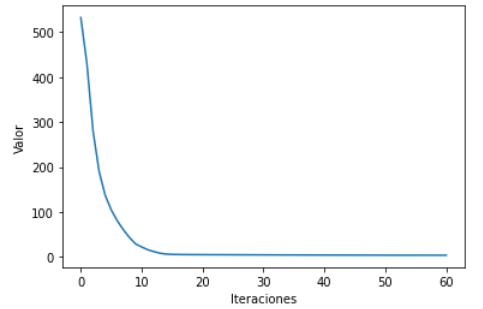
\includegraphics[scale=0.4]{e1-1.png}}
    \caption{Decremento de la función objetivo a través de las iteraciones, Rosembrock}
    \label{img-e1-1}
\end{figure}

\subsection{Algoritmo de Región de Confianza: Descenso de gradiente sobre el modelo}

En la tabla \ref{tab2} se muestra una comparativa del rendimiento del método con las dos funciones.
Nótese que los resultados obtenidos son para el mínimo local ya conocido para el caso de la función
de Rosembrock y al óptima para la función de Wood.

\begin{table}[htbp]
    \caption{Tabla comparativa del método usando descenso de gradiente sobre el modelo}
    \begin{center}
        \begin{tabular}{|c|c|c|c|}
            \hline
			\textbf{\textit{Función}}& \textbf{\textit{Iteraciones}}& \textbf{\textit{$||g_k||$}}& \textbf{\textit{$|f(x_k) - f(x^*)|$}} \\

            \hline
            Rosembrock& 352 & 9.9986 & 3.9866 \\
            Wood& 250 & 2.0000 & 4.2463e-13 \\
            \hline
            \multicolumn{4}{l}{}
        \end{tabular}
        \label{tab2}
    \end{center}
\end{table}

\begin{figure}[htbp]
    \centerline{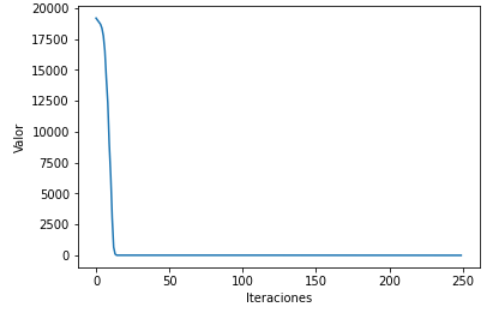
\includegraphics[scale=0.4]{e2-1.png}}
    \caption{Decremento de la función objetivo a través de las iteraciones, Wood}
    \label{img-e2-1}
\end{figure}


\subsection{Aproximación de histograma en 3D a través de funciones base radial con kernel gaussiano}

Se realizaron las pruebas sobre diversas grupos de imágenes, todos los histogramas se obtuvieron a
través del script en python brindado. Las siguiente imágenes muestran los mejores resultados
obtenidos para las imágenes.

\begin{figure}[htbp]
    \centerline{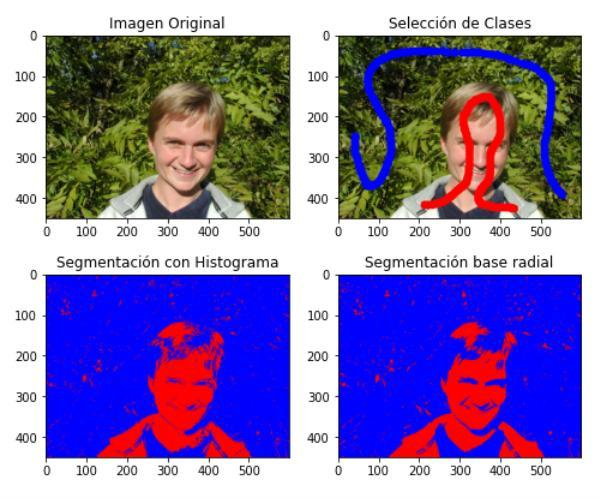
\includegraphics[scale=0.4]{1.jpg}}
    \caption{Segmentación a través del histograma y la aproximación a este, $bins=3$, funciones base = 30, $\sigma=20$}
    \label{img-e3-1}
\end{figure}

\begin{figure}[htbp]
    \centerline{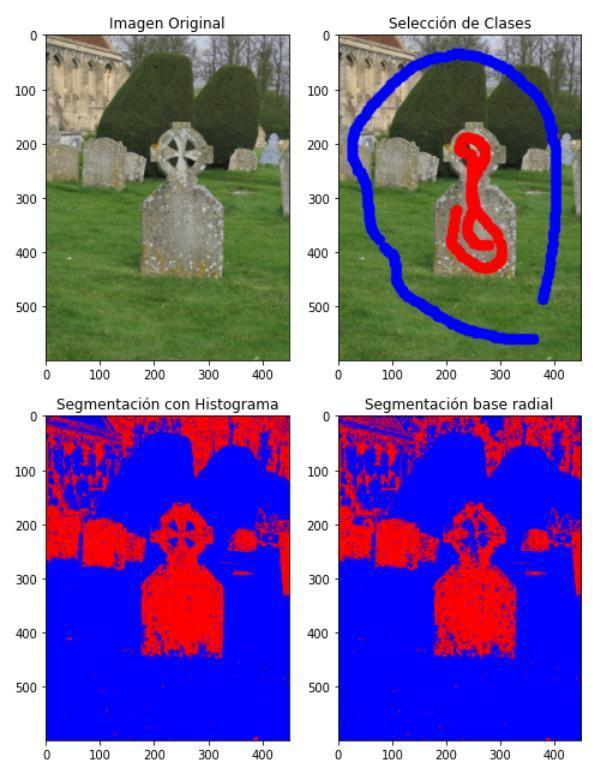
\includegraphics[scale=0.4]{2.jpg}}
    \caption{Segmentación a través del histograma y la aproximación a este, $bins=3$, funciones base = 30, $\sigma=0.1$}
    \label{img-e3-2}
\end{figure}

\begin{figure}[htbp]
    \centerline{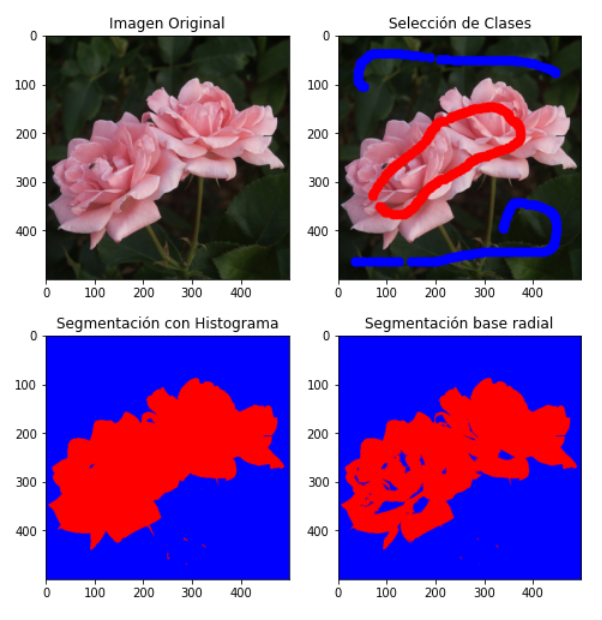
\includegraphics[scale=0.4]{3.png}}
    \caption{Segmentación a través del histograma y la aproximación a este, $bins=3$, funciones base = 30, $\sigma=0.1$}
    \label{img-e3-3}
\end{figure}

\begin{figure}[htbp]
    \centerline{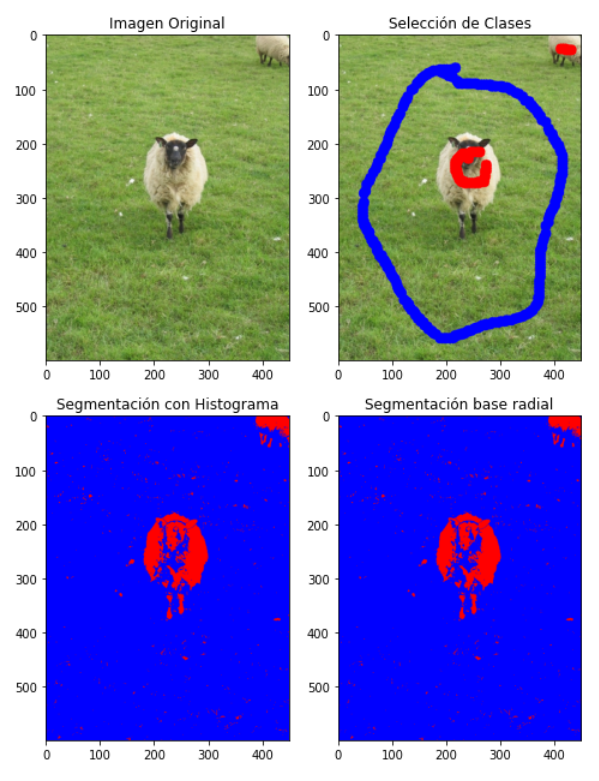
\includegraphics[scale=0.4]{4.png}}
    \caption{Segmentación a través del histograma y la aproximación a este, $bins=3$, funciones base = 30, $\sigma=0.1$}
    \label{img-e3-4}
\end{figure}


\section{Conclusiones}

Como se mencionó anteriormente en los métodos de región de confianza el cálculo del tamaño de paso y
la dirección de gradiente puede ser en diversas formas. En este caso se implementaron dos formas la
primera a través del método de Dogleg, el cual tratar de aproximar la trayectoria de la solución
mediante dos segmentos formados por el origen y el punto $p_k^U$ y de $p_k^U$ a el punto $p_k^B$.
La segunda forma fue interar sobre el modelo hasta encontrado un tamaño de paso y dirección valido
a través de descenso de gradiente sobre el modelo. Como se observa en los resultados la convergencia
del método de Dogleg es mucho más rápida que la segunda aproximación covergiendo al rededor de 60
iteraciones vs 300 iteraciones del método usando descenso. En este caso con ambos métodos no se pudo
obtener el mínimo óptimo llegando solo al local para la función de Rosembrock, y llegando al mínimo
óptimo para la función de Wood solo en el segundo método de para la obtención de $p_k$.\\

Para varias imágenes, las aproximaciones a los histogramas fueron similares, mostrando
imágenes segmentadas con muy pocas diferencias. Sin embargo, para poder alcanzar resultados buenos
la clave es encontrar valores de $\sigma$ que nos permitan aproximarla de la mejor manera. Por lo
regular con alrededor de 60 a 80 funciones base los resultados son bastante buenos. El número de
bins usandos para la generación de los histogramas es de 3, un número mayor de bins provoca un
incremento substancial en el tiempo de ejecución y convergencia (horas).


\section{Apéndice}

\subsection{Algoritmos}


\begin{algorithm}[]
    \SetAlgoLined
    \KwResult{$x_k$}
	$x_k$ <- Inicializar \\
    \While{$||g_k|| > tol$}{
		Calcular $p_k$ que minimize el modelo $m_k(p_k)$\\
		$\rho_k = \frac{f(x_k) - f(x_k + p_k)}{m_k(0) - m_k(p_k)}$\\
		\If{$\rho < \frac{1}{4}$}{
			$delta_k = \frac{1}{4} \Delta_k$\\
		}
		\ElseIf{$\rho > \frac{3}{4}$}{
			$delta_k = min(2 \Delta_k, \hat{\Delta})$\\
		}
		\If{$\rho \le \eta$}{
			$continue$\\
		}

		$x_k$ = $x_k$ + $p_k$\\
	}
    \caption{Algoritmo de Región de Confianza}
\end{algorithm}

\begin{algorithm}[]
    \SetAlgoLined
    \KwResult{$p_k$}
	$g_k$ <- Ingresar \\
	$B_k$ <- Ingresar \\
	$\Delta_k$ <- Ingresar \\
    \While{$||g_k|| > tol$}{
		$p_k^U = \frac{g_k^T g_k}{g_k^T B_k g_k}$ \\
		$p_k^B = - B_k^{-1} g_k$ \\
		\If{$||p_k^B \le \Delta_k||$}{
			$p_k = p_k^B$\\
		}
		\If{$||p_k^U \ge \Delta_k||$}{
			$p_k = p_k^U \frac{\Delta_k}{||p_k^U||}$\\
		}
		\Else {
			$a = ||p_k^B - p_k^U||^2$\\
			$b = 2 p_k^B (p_k^B - p_k^U)$\\
			$c = ||p_k^U||^2 - \Delta^2$\\
			$\lambda = \frac{-b +- \sqrt{b^2 -4ac}}{2a}: \lambda \in [0,1]$\\
			$\tau = \lambda+1$\\
			$p_k = p_k^U + (\tau - 1.0) * (p_k^B - p_k^U)$\\
		}
	}
    \caption{Método de Dogleg, cálculo de $p_k$}
\end{algorithm}


\begin{algorithm}[]
    \SetAlgoLined
	\KwResult{$p_k$}
	$j=0$\\
	$z_0 = 0$\\
	$d_0 = -\nabla m_k(z_0)$\\
	$g_k$ <- Ingresar\\
    \While{$||d_j|| \neq 0, j < J$}{
		\If{$||d_j^T B_k d_j \le 0||$}{
			$a = d_j^T d_j$\\
			$b = 2 z_j^T d_j$\\
			$c = z_j^T z_j - \Delta^2$\\
			$\tau = \frac{-b +- \sqrt{b^2 -4ac}}{2a}: \tau \ge 0$\\
			return $p_k = z_j + \tau d_j$\\
		}
		$\alpha_j = - \frac{g_k^T d_j + z_j^T B_k d_j}{d_j^T B_k d_j}$\\
		$z_{j+1} = z_j + \alpha_j d_j$\\
		\If{$||z_{j+1}|| > \Delta_k$}{
			$a = d_j^T d_j$\\
			$b = 2 z_j^T d_j$\\
			$c = z_j^T z_j - \Delta^2$\\
			$\tau = \frac{-b +- \sqrt{b^2 -4ac}}{2a}: \tau \ge 0$\\
			return $p_k = z_j + \tau d_j$\\
		}
		$d_j = -\nabla m_k(z_{j+1})$\\
		$j += 1$\\
	}
	$p_k = z_{j+1}$
	return $p_k$
    \caption{Descenso de gradiente sobre $m_k(p)$ para cálculo de $p_k$}
\end{algorithm}


\section*{}

\begin{thebibliography}{00}
\bibitem{b1} Jorge Nocedal, Stephen J. Wright, ``Numerical Optimization,'' Second Edition, Springer.
\end{thebibliography}

\end{document}
